%&latex2e


\documentclass[twoside,draft]{article}
\usepackage{latexsym,e-journal}

\usepackage[letterpaper]{geometry}
\usepackage[utf8]{inputenc}
\usepackage[english]{babel}

\usepackage{amssymb,amsfonts,amsmath}

\usepackage[perpage,symbol*]{footmisc}
\usepackage[final]{graphicx}
\usepackage{pstricks}
\usepackage{cite}

\usepackage[varg]{txfonts}

\oddsidemargin=-0.20in
\evensidemargin=-0.20in
\topmargin=-30pt

\textwidth=498pt
\textheight=646pt


\begin{document}

\renewcommand{\refname}{References}
\renewcommand{\tablename}{\small Table}
\renewcommand{\figurename}{\small Fig.}
\renewcommand{\contentsname}{Contents}


\twocolumn[%
\begin{center}
\renewcommand{\baselinestretch}{0.93}
{\Large\bfseries BACK TO COSMOS

}\par
\renewcommand{\baselinestretch}{1.0}
\bigskip
F. M. Sanchez, \ V. Kotov, \ M. Grosmann, \ D. Weigel, \ R. Veysseyre, \ C. Bizouard, \ N. Flawisky, \ D. Gayral, \ L. Gueroult\\
\par
\medskip
{\small\parbox{11cm}{%
To the memory of Sir Michael Atiyah\\

The ancestral concept of Cosmos is rediscovered through the idea of a Tachyonic
Grandcosmos Multibasis Computer, inversing the Anthropic Principle and reestablishing
the Laplace Determinism. The observed fine tuning between physical dimensionless
parameters is interpreted as relations between optimal calculation basis, announcing a
dramatic progress in computer software. Three type of mathematical constants are
considered: Large, Intermediate and close to unity. The famous Large Number problem is
resolved by Eddington's statistical theory and the gravitational Hydrogen Molecule model,
leading to the visible Universe horizon radius R $\approx$ 13.812 Gly. The extension of
the double cosmic correlation defines a Topological Axis using Euler-Napier constant e as
primary basis, confirming String Theory, Cartan-Bott periodicity and the 30 holic
dimensions corresponding to the simplest space-time-matter diophantine equation T$^2\!$ = L$^3\!$ = M$^5\!$ = N$^{30}\!$. This dimension n = 30 corresponds to the common time, about 10$^{58}\!$ s, given by
two mandatory dimensional analysis, interpreted as the Supercycle period. The visible
Universe wavelength 'Topon': 2G$\hbar$/Rc$^3\!$ $\approx$ 4 $\times$ 10$^{-96}\!$ m corresponds to $n \approx 2e^{e}$ and enters the 1D
mono-radial holographic extension of the Bekenstein-Hawking Universe entropy, implying
the critical condition, and breaking the Planck wall by a factor $10^{61}$ , justifying the Hawking
trans-planckian frequencies. The monochrome holographic extension leads to a
Grandcosmos, larger than the visible Universe by the same factor $10^{61}$ . A toponic
quantization justifies the Cosmos vastness in a scanned Universe, justifying the entropy
factor 1⁄4. This implies a tachyonic speed in the same ratio by respect to c, justifying the
Planck re-normalisation of the vacuum energy, independently checked by the Casimir effect.
The couple Universe-Grandcosmos is confirmed by a dramatic geo-dimensional analysis,
where Length, Time and Mass ratios are considered as unit vectors in a 3D Super-space. A
matter-antimatter $10^{104}$ Hz Oscillatory Bounce unifies standard Single Bang with steady-
state cosmology, but suppress Relativity in cosmology at large, reestablishing the Newton
Absolute Space realized by the Microwave Cosmic Radiation, while Kotov cycle defines a
quasi-absolute clock. This new scanning space-time structure is confirmed by single-electron
cosmology, connected with Kotov period, and relying Sternheimer Biological scale factor and
Atiyah constant, which appear as privileged computation basis, as well as e, $\pi$ and $a \approx 137.036$,
in liaison with the sporadic groups. The Atiyah constant enters dramatic ppb precision
relations with particle data. This unifies mathematics, physics, chemistry, biology and
philosophy. It is predicted that the future telescopes will find mature galaxies in the very far range,
instead of a Dark Space, ruining the standard evolutionary cosmology, ill-founded on an imperfect
Cosmological Principle.

%% TODO: Insérer axe topologique
}}\smallskip
\end{center}]{%


\setcounter{section}{0}
\setcounter{equation}{0}
\setcounter{figure}{0}
\setcounter{table}{0}
\setcounter{page}{1}


\markboth{Bizouard, Flawisky, Gayral, Grosmann, Gueroult, Kotov, Sanchez, Veysseyre. Back to Cosmos}{\thepage}
\markright{Bizouard, Flawisky, Gayral, Grosmann, Gueroult, Kotov, Sanchez, Veysseyre. Back to Cosmos}

\section{Introduction}
\subsection{Introduction: Deterministic Computation and Hierarchy Principle}
It was observed that the physical constants are tightly contrived, but only three dimensionless parameters: a, p, and $a_{G}$, are sufficient to explain the main structures of the world [1]. Two of them are precisely measured: the electric constant a $\approx$ 137.035999139(31) measured with 0.23 ppb precision and the proton-electron mass ration p $\approx$ 1836.15267245(75), known with 0.41 ppb precision. By contrast, the gravitational coupling constant a$_G\!$ was neither well defined nor measured, due to the relatively large imprecision on G measurement (10$^{-4}\!$).

One can read [1]: \textit{“For example, the size of a planet is the geometric mean of the size of the Universe and the size of an atom; the mass of man is the geometric mean of the mass of a planet and the mass of a proton. Such relationships, as well as the basic dependences on a and aG from which they derive, might be regarded as coincidences if one does not appreciate that they can be deduced from known physical theory, with the exception of the Universe, which cannot be explained directly from kwown physics.... This line of arguments, which is discussed later, appeals to the 'anthropic principle'.”}

The existence of relations that are not explained by known physical theories, is called 'fine tuning' phenomena. But as soon as it involves the observable Universe radius, it signals the existence of a more fundamental theory that must take into account the \textit{ancestral Cosmos concept, which, as Eddington claimed [2], must be permanent [3]}. Extending this to the spatial homogeneity, this leads to the Perfect Cosmological Principle, the very foundation of the steady-state cosmology.

But, as about 30 dimensionless parameters appear as 'free parameters' in the Particle standard model, a large majority of theorists believe rather they are due to chance, leading to a separation between Physics and Mathematics, not to speak of Biology. Through a so-called Anthropic Principle, a majority believe in the Multiverse conundrum, a multiplicity of sterile Universes [1].

The present article shows that \textit{Physics is a part of mathematics}, refuting the Multiverse Hypothesis by precise fine-tuning between main physical and biological parameters, involving main mathematical constants in particle physics: $\pi$,  e and $\gamma$, the Euler-Mascheroni constant. Also, these relations confirm the Super-string Theory and rehabilitates the tachyonic Bosonic String Theory.

\textit{A decisive point of physics is the energy conservation.} Theorists associate it with time uniformity, but a more logical explication is that cosmos is a computer, so Intelligent Life receive a justification: to help the Cosmos computation. This Inverted Anthropic Principle answers the first of all questions : why do one asks questions ? One proposes that the parameters are optimal basis in a deterministic Computing Cosmos, and they appear indeed in DNA characteristics, and three-point temperatures of Mammals and main molecules [3 and reference therein].

\textit{This reinstates the Laplace determinism}, involving non-local hidden variables, which identify with the Cosmos, so rejecting the Copenhagen statistical interpretation of quantum mechanics.

The fact that three parameters, out of about 30, are so clearly emerging means that Physics, and more generally Science, is hierarchic: \textit{one can progress in science without knowing the details of the underlying fundamental theory.}

So, when Dalton found whole numbers in chemical reactions, he was prefiguring the atoms and Chemistry. The same for Balmer, spectral lines and wave mechanics. The same for Mandeleiev, atomic masses and nuclear physics. Also, when Mandel found whole numbers in Biology, he was prefiguring Genetics. In the same manner, this article prefigures \textit{the fundamental theory which must be based on arithmetics,} indeed a characteristic of deterministic computation, which could proceed by optimal algorithms, so en lighting the above Hierarchy Principle.

This article is separated in 3 sections, corresponding to 3 classes of mathematical constants, the large, the intermediate and the small, close to unity.

The first section explains why, in the Computation Hypothesis, large numbers are necessary, so justifying at last the Cosmos vastness. In particular,  the most famous prime number of Hstory 2$^{127}\!$-1, and the Eddington's Large number = 136 $\times$ 2$^{256}\!$  are empathized. The second section will study the role of intermediate mathematical constants such as the Eddington's constant 137. The third Section involves mathematical constants, such as $\pi$ and $\gamma$.  By contrast, the optimal computation basis e is used all along, in particular as the primary basis of the Topological Axis Function f\{n\} = exp(2n/4), the secondary basis being 2, the simplest basis of all.

\section {Chapter1}
\subsection {Internal Fine Tuning and Canonical Large Numbers}
\markright{Your Full Names.  Short Title of Your Paper}

The most famous fine tuning implies cosmic quantities, but this is awkwardly called the `Double
Large Number Problem`. If it is a `problem` for standard evolutionary cosmology, it is a precious
clue in steady-state cosmology based on the Perfect Cosmological Principle (spatial and temporal
homogeneity) [3].
This Cosmic Fine-Tuning leads directly to a Gravitational Hydrogen model of the universe [3]
defining the Universe horizon radius $R = 2a_{G} \lambdabar_{e}$ , the factor 2 coming from the two atoms in
Hydrogen molecule, where 
\begin{equation}
\lambdabar_{e} = \hbar/cm_{e}
\end{equation} is the Electron Compton reduced wavelength, and the
gravitational coupling constant 
\begin{equation}
a_{G} = \hbar c/G \cdot m_{H} \cdot m_{p}
\end{equation}, so the speed c is eliminated. This conforms with
Coherent Cosmology which needs signal celerity far exceeding c. This gives R = 13,812 Gly, corresponding to a Hubble constant 70.790 (km/s)/Megaparsec, compatible with the
most recent measurement [4]: 72(3) (km/s)/Megaparsec, which confirms the value measured
directly by the 1a type novae, while the standard optimization of 6 parameters results in a lower
value of 9\%.
Let us associate the visible universe of mass M with a matter-wave, of wavelength $\lambdabar_{M} = \hbar /Mc = 4
10^{-96} m$. This `Topon` is close to the touchstone n = 30 of the Topological Axis, see Fig. 1,
corresponding to $n \approx 2e^{e}$ , to $0.01\%$ , The Topological Axis illustrates the function $f{n + 4} = f^{2}{n}$
and results from the imbrication of relations of the form 
\begin{equation}
\lambdabar_{e} /l_{micro} \sim (l_{macro} /\lambdabar_{e})^{2}
\end{equation}
, followed by 
\begin{equation}
l_{macro} /\lambdabar_{e} \sim (\lambdabar_{e} /l\prime_{micro} )^{2}
\end{equation}:
$$
\begin{array}{ll}
%
\displaystyle
\lambdabar_{e}/\lambdabar_{M} \sim (R/\lambdabar_{e})^{2} \sim (\lambdabar_{e}/ \lambdabar_{X})^{4} \sim \\[+8pt]  % 1st row
(\lambda_{CMB}/ \lambdabar_{e})^{8} \sim (\lambdabar_{e}/\lambdabar_{W})^{16} \sim (2r_{H} /\lambdabar_{e})^{32}\\% 2nd row
\sim (\lambdabar_{e}/ l_{Gl} )^{64} \sim (\lambdabar_{str} /\lambdabar_{e} )^{128} \sim 2^{256}\\% 3rd row
\end{array}
$$
where a string wavelength $\lambdabar_{str}$ , appears, with mass about 2 MeV. So, the correlation is eightfold,
including, apart the two ones above, three relations which have been independently reported [3].
The overall large number $2^{256}$ has an evident computational character, confirmed below by the
dramatic appearance of the Eddington Large Number, and allows to approach each physical length.
In particular, the relation $R/\lambdabar_{e} \sim (l_{CMB} / \lambdabar_{e})^{4}$ ties two cosmic lengths, the Hubble radius and the CMB wavelength by a relation incompatible with the standard evolutionary cosmology. Of this order of
magnitude, we infer rather precise relations. First, considering the cosmological neutrino
background (CNB), whose wavelength is defined by $(l_{CNB} / l_{CMB})^{3} = 11/4$, we have $$R/ \lambdabar_{e} \sim
( l_{CNB}^{2} / l_{CMB} \lambdabar_{e} )^{4}$$ to $1.7\%$. Second, with the Hydrogen radius $r_{H(0)} = a\lambdabar_{e}$ , we infer 
\begin{equation}
R/r_{H(0)} \sim (4 \prec l_{CMB} /r_{H(0)} )^{4}
\end{equation}
precise to $0.6\%$. One notes that the appearance of the neutrino field is conform
with the synthesis of the two main cosmologies, where the single Bang is replaced by a matter-
antimatter Oscillatory Bounce [5].
In particular, it was noted [1] that $a_{G}$ is of order $W^{8}$ , where W is the mass ratio W boson-
Electron. With the above R value, one observes the following more symmetrical relation involving
the other (neutral) weak boson Z, in the 0.01\% indetermination of W and Z:
$R/\sqrt{(\lambdabar_{p} \lambdabar_{H})} \approx (WZ)^4$
where $\lambdabar_{p}$ and $\lambdabar_{H}$ are the Proton and Hydrogen reduced wavelengths. The precision of this formula
will be pulled to the ppb range in Chapter 3, by intervention of canonical mathematical constants.
The gravitational Hydrogen molecule model [3] implies the following double correlation,
which is the simplest case of Eddington's statistical theory [2]. The position of a `reference particle`
is supposed to be determined with an uncertainty ${R/2}$. For N particles of mass m components of the visible Universe, the deviance is statistically divided by $\sqrt{N}$, where $N = M/m$. If m is assumed to be
the effective mass of the electron in the Hydrogen atom, $m\prime_{e} = m_{e} p/H$, and if, moreover, we equate
the deviance $R/(2\sqrt{(M/m\prime_{e}))}$ to the Hydrogen wavelength $\lambdabar_{H} = \hbar/c \cdot m_{H}$ , one obtain the double relation:
$$R/2\lambdabar_{H} = \sqrt{(M/m\prime_{e})} = \frac{\hbar \cdot c}{G \cdot m_{e}\cdot m_{p}}$$
This is the definitive interpretation of the Double Large Number Fine-tuning. So, while the two
pillars of Physics, Relativity and Quantum Theory are unable to conciliate Gravitation and Particle
Physics, the third pillar, Statistical Physics, directly makes this connection in cosmology [2].
Recall that, contrary to what is often stated, Quantum Physics does not limit to Micro-physics.
Indeed the exclusion principle applies in both solid state physics and in stellar physics. In particular,
for a star containing N s atoms, in which the pressure has reached the quantum degenerancy value
(case of white dwarfs), exclusion principle applies for electrons, and the radius star is about $R/N_{s}^{1/3}$ .
So the formula giving the Hubble radius R, a very difficult measurement which puzzled a whole
century, was already contained in astrophysics textbooks. The universe radius amazingly appears as
the limit of a mono-atomic star radius, of which the electrons are in degeneracy state. Eddingon was
aware of this Cosmologic Exclusion Principle, but could not conclude since, at his epoch, the
Hubble measurement for R was false by an order of magnitude.
The reason for this discrepancy is that Lemaitre and Hubble considered galaxies of the Local
Group, which do not participate the so-called Space expansion. In fact, it suffices to introduce a
repulsive force proportional to galaxy groups separation distance, for explaining the canonical
exponential recession. There is no need of the so-called `dark energy`, the repulsive force is simply
the cosmological constant identified to $1/R^{2}$ . The distance for which this force exceeds attractive
gravitation between galaxies is about $10^{6}$ light years \cite{fm1}[3], which corresponds, in the Topological
Axis, to the Atiyah Constant $\Gamma$ , presented in the Section III, see Fig 1.
In the steady-state cosmology, such a repulsive force between galaxy groups is necessary, in
order to avoid a big chill due to the thermodynamics second principle. But, inside a galaxy group,
another evacuation mechanism must occur: it would be the role of massive black holes.

\begin{figure}
\centering
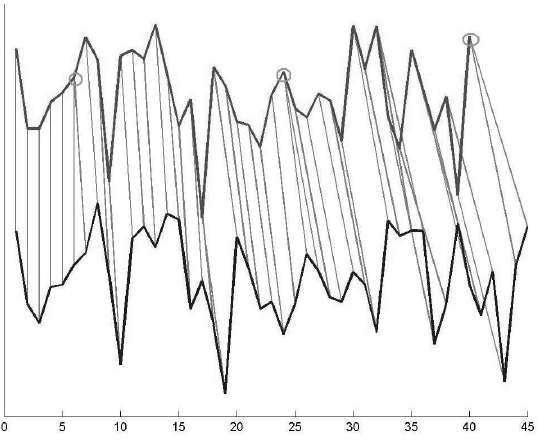
\includegraphics[width=8cm,height=6.5cm]{./figures/figure}
\caption{The Topological Axis.}
\label{fig:figure_label}
\end{figure}

\subsection{Cosmic Holography, Toponic Quantification and Cosmos vastness}

In the steady-state cosmologic model of Bondi, Gold and Hoyle\cite{bondi}, the Perfect Cosmological
Principle implies the invariance of the Universe mean mass density $\rho$ and the exponential recession
of galaxy groups, with time constant R/c being compensated by the appearance of m n massive
neutrons at rate $c^{3} /Gm_{n}$. The invariant visible Universe radius R is then defined by the
Schwarszchild relation so that each point is the center of an equivalent R-radius black hole, of
critical mass $M = Rc^{2} /2G$ and wavelength $\lambdabar M = \hbar/Mc = 2l_{P}^{2} /R$, the above `Topon`. The Bekenstein-
Hawking entropy of this black-hole Universe shows an 1D extension of the standard Holographic
Principle , only devoted to 3D application \cite{bousso}[6]:
$S_{BH} = \pi(R/l_{P})^{2} = 2\pi R/\lambdabar_{M}$
where $l_{P} = (G\hbar/c^{3} )^{1/2}$ is the Planck's length. Let's not forget, while the standard evolutionary cosmology
use differential equations, the steady-state Cosmology must favor such integral relations. This one
uses the Archimedes Testimony tying the Disk Area to its Perimeter.
In the standard evolutionary view, the observed homogeneity of causally disconnected regions
of space is known as the so-called `horizon problem`, and is at the origin of the awkward inflation
hypothesis, which is not necessary in the steady-state model. Indeed, the critical condition is
furnished by the above very definition of R.
The cosmic wavelength $\lambdabar_{M} \sim 10^{-95} m$ breaks `Planck's wall` by a factor $l_{P} /\lambdabar_{M} \sim 10^{61}$ : hence why this holographic relation went unnoticed for decades. Indeed, it was admitted that $l_{P}$ was the quantum of Space: in fact Planck's length is only an intermediate holographic length.
The gravitational potential energy of a critical homogeneous sphere is $-(3/5)GM2/R = -
(3/10)Mc^{2}$, while the nonrelativistic kinetic energy of galaxies is $(3/10)Mc^{2}$. Their sum is therefore
zero: the density of the so-called `dark energy` being compatible with 7/10, this dark energy is a
trivial false problem. As recalled above, Relativity is a local theory that does not apply in
Cosmology: galaxies actually reach speed c, and crossing the horizon, reach a Grandcosmos of
radius $R_{GC}$ , given, as a first approximation, by the symmetrical holographic relation, this time
monochrome instead of the monoradial relation above:
\begin{equation}
S_{BH}\, = \pi(R/l_P )^{2} = 2\pi R_{(0)} GC /l_{P}
\end{equation}
with $R_{(0)} GC /R = l_{P} /\lambdabar_{M} \sim 10^{61}$ . The conservation of the time constant $t = R/c, = R_{(0)} GC /C$ introduces a canonical velocity $C \sim 10^{61} c$, lifting the veil on an energy larger than that of the visible Universe by a
factor $10^{122}$ , which can be identified with the $l_{P}$ -normalised quantum energy of vacuum, checked by
the Casimir effect [7]. The central problem of quanto-cosmic physics is thus solved. Moreover, the
objections against the Hawking approach using trans-plankian frequencies are wiped out [8].
In a better approximation, justified below, R is replaced in the above relation by $R\prime = 2\hbar^{2}/Gm_{N}^{3}
\approx 18.105 Gly$, where $m_{N} = am_{e}$ is the Nambu mass, of central importance in particle
physics. Indeed, the half radius $R\prime/2$ has a simpler definition than $R/2$: it corresponds to the
elimination of c between the classical electron radius and the Planck length. In this way, the sphere
of radius $R\prime$ appears as the spherical hologram representation of the outer Grandcosmos:
\begin{equation}
S\prime_{BH}\, = \pi(R\prime/l_{P})^{2} = 2\pi R_{GC} /l_{P}
\end{equation}
This value will be dramaticaly confirmed in the section I.IV.
Assuming the Toponic Quantification Hypothesis, the mass of a particle is an exact sub-multiple
of the mass-equivalent M of the visible Universe: $m = M/N_{m}$ , and its canonical wavelength is $N m \lambdabar_{M}$ ,
allowing the following holographic extension of the above mono-radial holographic conservation:
\begin{equation}
S_{BH}\, = \pi(R/l_{P})^{2} = \frac{2\pi \cdot R}{\lambdabar_{M}} = \frac{2\pi \cdot N_{m} \cdot R}{\lambdabar_{m}}
\end{equation}
This series of large circles generates, by scanning, the approximation of a sphere: one thus passes
from the Disk to the Sphere. Note that this justifies the factor $\frac{1}{4}$ in above BH entropy. But, for
the approximation to be sufficient, the numbers $N_{m}$ must be very large. In this way, the Cosmos-
Computer can use the computational properties of the mathematical constants of the continuous
analysis, such as $\pi$ (See Section 3).
The immensity of the Cosmos thus receives a much simpler computo-holographic explanation than
that of standard cosmology, where initial conditions, during Planck's time, would be adjusted with
extreme precision, even with inflation. By identifying the large number of Eddington $N_{Ed} = 136 \cdot
2^{256}$ as the equivalent number of neutrons in the effective mass $\frac{3M}{10}$ this leads to $R \approx 13,805
Gly$ at $0.05\%$of the above value.
In the Hydrogen gravitational molecule model, R is defined by the following 1D-2D-3D Special
Holographic Relation, where the wavelengths of the Electron, Proton, and Atomic and Molecular
Hydrogen apear, as well as that of the background radiation
$2 \pi R/\lambdabar_{e} = 4 \pi \lambdabar_{p} \lambdabar_{H} /l_{P} 2 \simeq (4\pi/3)(\lambdabar_{CMB} /\lambdabar_{H2})^{3}$
The above relation gives $T_{CMB} \simeq 2.73 K$. With the measured temperature of the cosmic
background, there is a gap compatible with $(H/p G ) 2 p/6\pi_{5} $, where $p_{G}^{2} = P^{2} /2^{127}$ , with $P = \lambdabar_{e} /l_{P}$, . 
This eliminates $l_{P}$ , so gives a relation independent of G:
$$2^{127} = 2\pi^{2} \lambda_{CMB}^{3} /\lambdabar_{e} \lambdabar_{H} 2$$
=> $\Theta_{CMB} = 2.725820805 K$ which is the surface of the 4-sphere of radius $\lambda_{CMB} / \lambdabar_{m}$, where $\lambdabar_{m} = (\lambdabar_{e} \lambdabar_{H} 2 )^{1/3} $, proving the relevance of
the Lenz-Wyler approximation for the Proton/Electron mass ratio $p = 6\pi^{5}$ , (see Section 3). Recall
that $2^{127} - 1$ is the most famous prime number in the history of Mathematics, being the last term of
the Combinatorial Hierarchy of Special Numbers of Mersenne 3, 7, 127, the sum of which is 137.
The critical mass is related to the elementary masses by:
\begin{equation}
m_{P}^{4}\, = M m_{e} m_{p} m_{H}
\end{equation}
this directly involves Planck's mass $m_{P}$ , which at this day, has no known application, except
that it is close to the mass of the human ovocyte. In this way, the local inertia is related to the distant
masses, in accordance with the Mach principle, which the Relativity Theory does not explain.
Another shortcoming of this theory is that it does not define any inertial frame. However, the
Doppler dissymmetry of the cosmic background indicates the speed of our local group of galaxies:
630 km/s. The cosmic background is therefore tied to the Newton absolute frame, the Grandcosmos.
The mathematical continuity being excluded by the above Calculative Principle, the associated
time 
\begin{equation}
\lambdabar_{M} /c = 1.33 \times 10^{-104}s
\end{equation}
is the new candidate for the `Chronon`, the `quantum of time`, so the
oscillatory bounce has a frequency about $10^{104}Hz$ \cite{fm2}[5].

\subsection{Evidence for Tachyonic Flickering Space-Time-Matter}

The tachyonic hypothesis is consistent with the non-local character of quantum mechanics. The
following considerations and observations confirm this hypothesis.

\subsection{Single Electron Cosmology}

The single-electron cosmology [3] uses the electron indeterminacy, which is the real basis of the
Exclusion Principle, giving an horizon value R 1 only dependent of the Hydrogen radius $a\prime = aH/p$. It
is the value for which the mean cosmic value is also the atomic one:
\begin{equation}
\frac{\sum(1/n)}{\sum(1/n^{2})} = a\prime
\end{equation}
with the sum running from 2 to $R_{1} /\lambdabar_{e}$. This implies:
$R_{1} = \lambdabar_{e} exp((\pi^{2} /6 - 1)a\prime + 1 - \gamma) \approx 15.77465 Gly$
very close (0.4 ppm) to the following expression, where $p_{G} = P/2^{127}/2$ , and $\beta = (H - p)^{-1}$ is the
Rydbergh correction factor and $p_{0} = 6\pi^{5}$ the Canonic Lenz-Wiler Approximation of p:
\begin{equation}
R_{1} = ( p_{0} /p_{G} ) \sqrt{(\beta R R\prime)}
\end{equation}

Now, with the Kotov length $l_{K} = ct_{K}$ , see below, one notes that $\sqrt{(\frac{R}{a_{w} l_{K}})}$ is close to $\sqrt{a}$, while
the replacement of R by $R_{1}$ is about $4\pi$ , the canonical form for $\sqrt{a}$, the deviation being compatible
with $p/p_{0}$ , where $p_{0} = 6\pi^{5}$ is the Lenz-Wyler approximation for p (Section 3.1):
$$\sqrt{(R_{1} /a_{w} l_{K})} \approx frac{4\pi^{p}}{p_{0}} \Leftrightarrow t_{K} \approx 9 600.591445 s$$ a relation independent from G. 

This $t_K$ value will be confirmed, in the ppb range, by the value
deduced from $t_{K} /t_{e} = \sqrt{(a_{G} a_{w})}$, see below, using values of $a_{w} and a_{G}$ connecting, again in the ppb
range, with $\Gamma$, the Atiyah Constant (section 3.5).
From the Holographic two-step interaction [3], it was deduced that the Kotov period is
associated with the photon mass. With the above value, it is $$m_{ph} = \lambdabar/c^{2} t_{K} \approx 1.222 \times 10^{-55} kg$$, the
graviton mass being: 
\begin{equation}
m_{gr}\, = m_{ph} /a_{w} \approx 3.722 \times 10^{-67} kg
\end{equation} 
The corresponding ratios with electron mass(Fig.1) corresponds respectively to n = 24 and $n = \Gamma$ , the Atiyah constant, see Section 3.8.

\subsection{The Kotov Cosmic Coherent Oscillation Period}

The Kotov non-Doppler cosmic oscillation \cite{Lyuty} is not considered seriously, since it seems to
violate the most basic prerequisite of physics, the generality of Doppler phenomena. Interpreting
this as a tachyonic phenomena, we identified the Kotov period $t_{K} \simeq 9600.06(2) s$, taking the electron
characteristic time $t_{e} = \lambdabar_{e} /c$ as unit, to the simplest relation eliminating c between $a_{G}$ and $a_{w}=
\hbar^{3} /G_{F} m_{e}^{2} c$, the well measured $10^{-7}$ dimensionless electroweak coupling constant $a_{w}$ :
\begin{equation}
t_{K} / t_{e} = \sqrt{(a_{G} a_{w})}
\end{equation}
The weak coupling constant [1] $a_{w} = (E_{F} /m_{e} c^{2} )^{2}$ is defined from the Fermi energy 
\begin{equation}
E_{F} \approx 292.806161(6) GeV \approx 573007.33(25) m_{e} c^{2}
\end{equation}, itself tied to the weak force constant 
\begin{equation}
G_{F} \equiv (\hbar c)^{3} /E_{F}^{2} \approx
1.4358509(7) \cdot 10^{-62} Joule \cdot m^{3}
\end{equation}
\cite{Pdc}. This introduces the product of two area speeds, confirming the
flickering hypothesis:
\begin{equation}
(\lambdabar_{e} 2/t_{K} )(hbar/\sqrt{(m_{p} m_{H})})\, = \sqrt{(GG_{F})}
\end{equation}
so the best measured cosmic quantity, the Kotov period, implies a symmetrization between
gravitation and weak nuclear force. This specifies the G value to $10^-{6}$ precision (ppm). It is
compatible with the well-elaborate $10^{-5}$ BIPM measurement \cite{Quinn}, at several sigmas from the Codata
value [10], but the later is the mean between discordant measurements.
Computer analysis shows that this value of G is compatible with the well-defined following
value, with $m_{P} \equiv (\hbar c/G)^{1/2}$ and $d_{e} \approx 1.001159652$ the relative electron magnetic moment :
\begin{equation}
(2^{127} /a_{G} )^{1/2} \approx d_{e} (H/p)^{3}
\Leftrightarrow G \approx 6.6754552 \times 10^{-11} kg^{-1} \cdot m^{3} \cdot s^{-2}
\end{equation}
This value will be confirmed, in the ppb range, in Section III.

\subsection{The omnipresence of the Kotov cycle in astrophysics}

With $t = R/c$, the relation $(t t_{K2} )^{1/3} \approx 10.8$ years, compatible with the famous 11 years sun period
was noted. It was proposed that this unexplained phenomena, responsible for moderate periodic
climate variation, was also of flickering cosmic origin [12]. This hypothesis has been recently
confirmed by the straight temporal profile of the phenomena, showing it is tied to a quantum
process \cite{Kotov}.
This Kotov perodicity implies a moderate climate variation. Now, a much larger one, involving
glaciations, is tied to the Milankovitch period (100000 years), which presents also a straight
temporal edge. Moreover, these two periods seem to be tied to the dimensions n = 24 and $\Gamma \approx 25$,
characteristics respectively of a stellar system and a galaxy, see Fig.1. As the second period was
attributed to an earth orbital oscillation due to Jupiter effects, this suggests that the solar system is
tied to cosmic influence. Indeed, the Kotov period shows itself rather particular in the solar system.
In particular, the Uranus orbital radius is very close to the Kotov length $l_{K} = ct_{K}$ .
Remarkable enough, a `mysterious` period $\approx 1/9$ days of the Sun's pulsations has been predicted
long before its actual discovery in 1974. Namely, 73 years ago, French amateur astronomer Sevin
(1946) claimed that « la periode propre de vibration du Soleil, c'est-a-dire la periode de son infra-
son (1/9 de jour), a joue un role essentiel dans la distribution des planetes superieures». Presumably,
the Sevin's «vibration period» of the Sun was merely an issue of his reflections about resonances
and distances inside the solar system. Nevertheless, solar pulsations with exactly that period were
discovered, after decades, - and independently of the Sevin's paper, - by a few groups of
astrophysicists. Soon the presence of the same period, or timescale, was found in other objects of
Cosmos too (see Kotov, 2018, and references therein) .
Opponents emphasize often that $t_{K}$ is very close to the 9th harmonic of the mean terrestrial day: the corresponding ratio - of the length of a day to the $t_{K}$ period - is equal to 8.99943(1), - and claim
thus the $t_{K}$ oscillation of the Sun should be regarded as an artifact (see, e.g., Grec and Fossat, 1979;
Fossat et al., 2017). As a matter of fact, however, the $t_{K}$ period occurs to be the best commensurate
timescale for the spin rates of all the most massive and fast-rotating bodies of the solar system, in
general.
This is obvious from Fig. 2, which shows the resonance spectrum $F( \nu )$, calculated for 15
motions of 12 largest, fast spinning, objects of the system (with the mean diameters $\geq 500$ km and
periods < 2 days: six planets, three asteroids and three satellites, leaving apart trans-neptunian
objects; see Kotov, 2018). The peak of the best commensurability corresponds to a period of
9594(65) s, which coincides well, within the error limits, with $t_K$ at about $5.3 \theta$ C.L., i.e. with a
chance probability $10^{-7}$ .
It seems very puzzling also that the spatial scale $t_{K} \approx 19.24 A.U.$ occurs to be the best
commensurate with orbital sizes of the main planetary orbits of the solar system, - see Fig. 3,
where the resonance spectrum $F( \nu )$ is plotted for 11 orbits, including those of asteroid belt, Pluto
and Eris (orbital «diameters» were approximated by the major axes, and for the inner orbits they
were multiplied by $\pi$). The primary peak - of the best commensurability - corresponds to the
spatial scale 9600(120) light sec., or 19.24(3) A.U., at $4.7 \theta$ C.L. (Kotov, 2013)
Close binaries are characterized by the $t_{\Theta}$ resonance too, with the $\pi$ number as a factor of ideal
incommensurability of motions, or frequencies (Kotov, 2018). Fig. 4 shows the resonance spectrum,
or metrics of motion, $F_{1} (\nu) \equiv F(\pi \cdot \nu/2)$, computed for 5746 close binaries, including cataclysmic
variables and related objects. The major peak, with C.L. of about $7 \theta$, corresponds to the timescale
9590(70) s, coinciding within the error limits with $t_{K}$ (the stellar data were taken from all available
binary stars catalogues and original papers).
To compute the $F_{1} (\nu)$ spectrum, the program finds - for each test frequency $\nu$ - deviations of
ratios $(2\nu_{i} /\pi \nu) k \geq 1$ from the nearest integers, and determines then the least-square minimum of such
deviations. Here $\nu$ is the test frequency, $\nu_{i}$ minus the frequency of a given object, i = 1, 2, ...N - the
ordinal number, with N, the total number of observed periods in a sample of objects, and the power
k = 1 or -1. The factor of two in Eq. (2) takes into account that second half of the orbit repeats the
first one, and the transcendental number $\pi$ appears as a factor of orbital stability, or «ideal»
incommensurability, of motions, or frequencies (the $\pi$ number, in fact, characterizes geometry of
space; for details see Kotov, 2018).
Recently it was shown, that the $t_{\Theta}$ timescale characterizes, statistically, the motion of superfast
exoplanets too, see Figure 5.
It was shown in fact, that a number of superfast, with periods < 2 days, exoplanets revolve
around parent stars with periods, near-commensurate with timescales $t_{1}$ and/or $2 t_{1}/\pi$, where $t_{1} =
9603(85) s$ agrees fairly well with the period $t_{K} \approx 9600$ s of the so-called «cosmic oscillation», found
firstly in the Sun, then - in other variable objects of the Universe (the probability that the two
timescales would coincide by chance is near $3 \cdot 10^{-4}$).

\begin{figure}
\centering
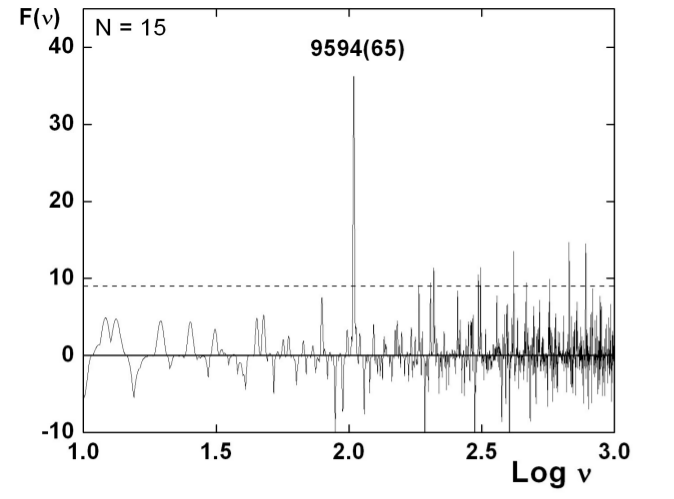
\includegraphics[width=8cm,height=6.5cm]{./figures/figure1}
\caption{Resonance-spectrum $F(\nu)$ computed for 15 motions of the largest, fast-spinning bodies of
the solar system. On horizontal axis is logarithm of frequency $\nu$ in $\mu$Hz, the dashed horizontal line
shows a $ 3 \theta $ C.L., and the primary peak yields to the best - commensurable period 9594(65) s.}
\label{fig:figure_label}
\end{figure}

\begin{figure}
\centering
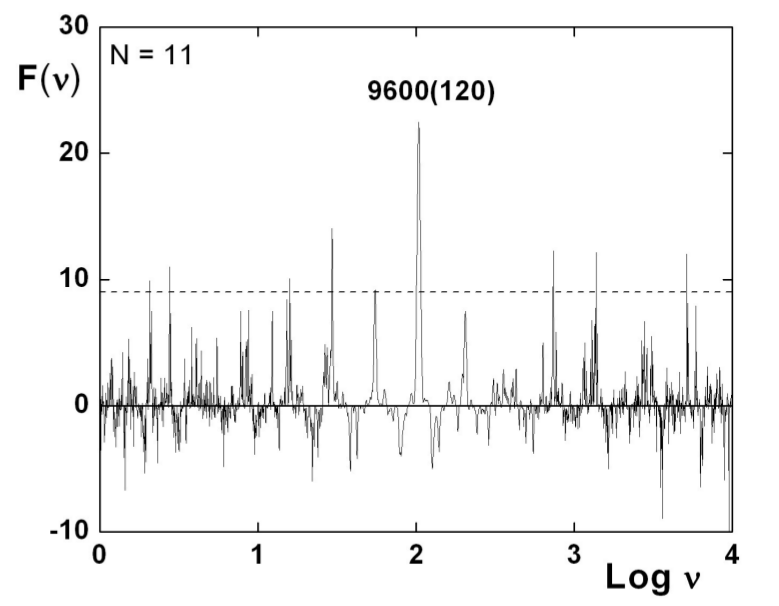
\includegraphics[width=8cm,height=6.5cm]{./figures/figure2}
\caption{Same as Fig. 2, for N = 11 sizes `diameters` of the solar system (with c = 1 and the $\pi$
factor for inner orbits). The highest peak corresponds to the spatial scale 9600(120) light sec.}
\label{fig:figure_label}
\end{figure}

\begin{figure}
\centering
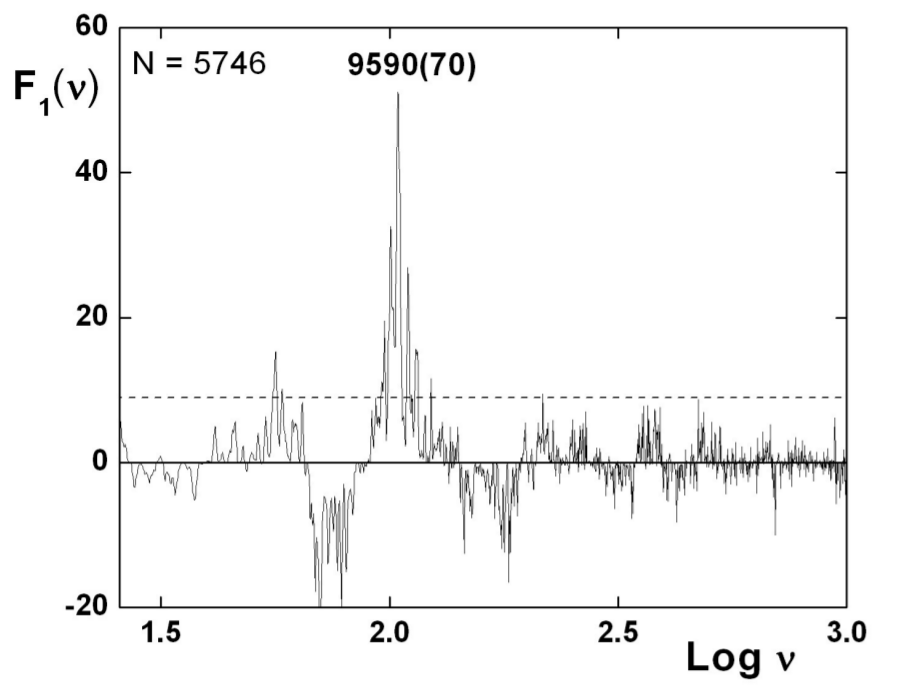
\includegraphics[width=8cm,height=6.5cm]{./figures/figure3}
\caption{Resonance-spectrum $F_{1} ( \nu)$, computed for N = 5746 binaries with periods < 5 days.
Horizontal axis gives logarithm of the trial frequency $\nu$ in $\mu Hz$, the dashed line indicates a $3 \theta$
C.L., and the major peak corresponds to a timescale of 9590(70) s.}
\label{fig:figure_label}
\end{figure}

\begin{figure}
\centering
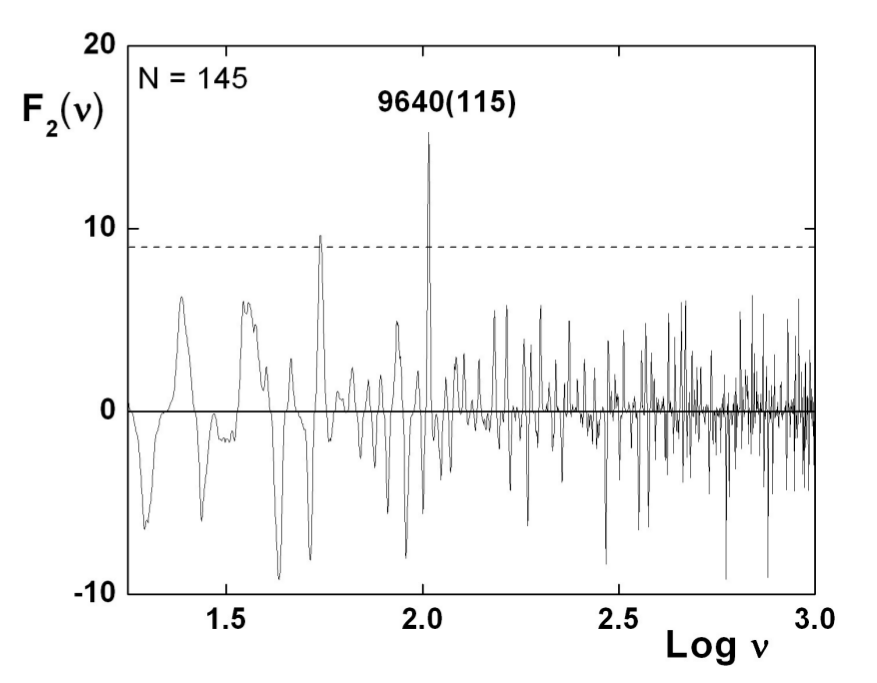
\includegraphics[width=8cm,height=6.5cm]{./figures/figure4}
\caption{Same as Fig. 4, for the $F_{2} ( \nu )$ spectrum, computed for N = 145 exoplanets with P < 1.5
days. The strongest peak of the composite commensurability corresponds to a period of 9640(115) s
at nearly $3.9\theta$ significance (after Kotov, 2018).}
\label{fig:figure_label}
\end{figure}


\subsection{The Tifft, Arp and Pioneer effects}

Another unexplained effect is the 75(5) km/s periodicity in the galactic redshift [14]. If one considers
velocity $v_{1}$ as being compatible with $\frac{c}{v_{1}} \approx \sqrt{a_{w} /a} = \frac{F}{a}$, corresponding to the quantum resonance $$\nu_{n} = nv_{1} =n\hbar /r_{e} m_{F} $$, where $r_{e} = \frac{\lambdabar_{e}}{a}$ is the electron classical radius and $m_{F} = m_{e}\sqrt{a_{w}}$ is the Fermi mass, close to the mean DNA nucleotide mass \cite{fm1}.
The Halton Arp observations of chains of galaxies with different redshifts [15] was also
rejected. But it could be the sign of the galactic regeneration constantly maintaining the visible
Universe mass: this is confirmed by the following confirmation of the invariance of the mean mass
density $\rho_{c}$ .
Much controversial is the Pioneer deceleration [16] $$g_{Pi} \approx 8.7 \times 10^{-10} ms^{-2}$$. It fits with
the Pioneer time $$t_{Pi} = c/g_{Pi} \approx 3.4 \times 10^{17} s$$, close to $$t = R/c \approx 4.3587 \times 10^{17} s$$. The following section will show a connexion between the Kotov, Tifft and Pioneer effects.

\subsection{The intriguing Logic of Prospective Dimensional Analysis}

Physical relations use principally physical quantities as monomials of type $Q = M^{x} L^{y} T^{t}$ , where
the three categories, M, L and T are Mass, Length and Time measurements, and where the exponents are
rational numbers. However, the addition of measures of different categories has no signification.
This seems at first sight illogical, since, fundamentally, a product is a sum of additions. So there
must be a hidden common nature for the 3 categories, mass, length and time. This sustains the
above single electron cosmic model [3]. Moreover, this mimics the Fundamental Principle of
Arithmetics, founded on prime numbers, but limited to the three M, L and T categories. Indeed, with $t =
R/c$, summing the square of $ln(M\prime/m_{e} )$, where $M\prime = R\prime c 2 /2G$ is the critical mass in the above
holographic sphere representing the Grandcosmos, and the square of $ln(R/\lambdabar_{e} ) = ln(t/t_{e} )$, one gets, to
40 ppm:
\begin{equation}
ln 2 (M\prime/m_{e} ) + ln 2 (R/\lambdabar_{e}) + ln 2 (t/t_{e} ) \approx ln 2 (R_{GC} /\lambdabar_{e} )
\end{equation}
more precisely, to $10^{-8}$ , corresponding to $10{-7}$ precision on the above G value:
\begin{equation}
ln(\sqrt{(ln 2 (M\prime/m_{e} )} + ln 2 (R/\lambdabar_{e} ) + ln 2 (t/t_{e} ))) \approx 2e - 1/2a
\end{equation}
This is a dramatic geometrical confirmation for the visible Universe - Grandcosmos holographic
couple.
Another crucial point in Physics is the existence of invariant fundamental constants. Thus,
association of three of them must give characteristic values of M, L, T. So, approaching a domain in
Physics necessitates to calculate characteristic values (M, L, T), from the three universal constants
which are the most pertinent in the considered domain. This Prospective Dimensional Analysis is
largely used in Fluid Mechanics, were the equations are intractable, but is largely ignored in other
domains, because there is no real mathematical foundation, apart the above essential remarks. But
in virtue of the above Hierarchy Principle, the lack of theoretical justification is not a reason to
neglect Prospective Dimensional Analysis.
Now, the elimination of c in the above R formula means that the simplest basic dimensional
analysis starting from $\hbar$, G and m, the Electron-Proton-Neutron mean mass gives a good
approximation for R/2. Indeed, in the Hypothesis of a Coherent Cosmos, it is logical to discard c
which is far two small a speed. This has not been observed during one century, since c is always
believed to be the single mandatory foundation of Space-Time. The warning of Poincare, the true
discoverer of Relativity: `use 4D space but do not confound Space and Time` has long been
forgotten, and physicist have unwisely put c = 1 in their equations.
In his three first minutes of cosmology, one of the author obtained the length:
\begin{equation}
l (\hbar,G,m) = \hbar 2 /Gm^{3} \approx R/2
\end{equation}
but it took 9 years to nurture this publication [12], and it appeared later [3] that m must be considered more precisely as the cubic root of the product 
\begin{equation}
m_{e} \cdot m_{p} \cdot m_{H}
\end{equation}. Moreover, the above critical condition
links the time $t = \frac{R}{c}$ and the mean mass density by the c-free formula:
\begin{equation}
\rho_{c} = 3/8\pi Gt^{2} \approx 9.41198 \times 10^{-27} kg \cdot m^{-3}
\end{equation}
, So the mainstream idea of a temporal variability of the mean density $\rho_{c}$ cannot be to
sustain, meaning that $\rho_{c}$ must be considered as a fundamental constant. One writes:
\begin{equation}
t{\hbar,\rho_{c} ,G}\, = 1/\rho_{c}^{1/2} G^{1/2} = (R/c) (8\pi/3)^{1/2}
\end{equation}
This idea of $\rho_{c}$ being a fundamental constant permits to define R without any ambiguity: the
radius containing a critical mass. This means each point is the center of an equivalent black hole,
justifying the above application of the Bekenstein-Hawking entropy. Opponents would say that the
center of a black hole presents a singularity: that is indeed the case in the above flickering Space-
Mass-Time hypothesis. Other will argue that the flying galaxies cannot reach the celerity c at
horizon, but it must be reckognized that Relativity is a local theory, so do not apply in Cosmology.
Indeed, even General Relativity in unable to define what is a Galilean frame, while the Foucault
pendulus shows it directly, realizing the Cosmic Microwave Background frame, identified with the
Grandcosmos frame, as seen above.
Introducing the Fermi constant $G_{F}$ , the associated c-free length is very particular, to $1.7\%$:
$$l{\hbar,\rho_{c},G_{F}} = \hbar/\rho_{c}^{1/2} G_{F}^{1/2} \approx 9.07154 10^{9} m \approx \lambdabar_{e}^{2}/l_{P}$$
Now, the following mandatory c-free times are close each over to $0.7\%$:
\begin{equation}
T{\hbar,\rho_{c} ,G_{F} }\, = \hbar^{4} /\rho_{c}^{3/2} G_{F}^{5/2} \approx 5.4829 \cdot 10^{57} s
\end{equation}
$$T\prime{\hbar,G,m} = \hbar^{3} /G^{2} m^{5} \approx 5.5224 \times 10^{57} s$$
This would be the periodic time of a Large Cosmologic cycle, which matches with Topological Axis at n = 30;
the holic dimension (see below), to 4\%. Comparing T with the Kotov Non-Doppler Cosmic
Oscillation period $t_{K} \approx 9600.60(2)$ s, one observes, to $0.04\%$:
$$T/t_{K} \approx O_{M} /\sqrt{2}$$
where $O_{M}$ is the cardinal order of the Monster Group, the largest of the 26 sporadic groups, which is
suspected by some researchers to play a central role in Physics: indeed string theory allows a bridge
between apparently no-connected mathematical theories \cite{Borcherds}[17]. The simplest interpretation of T is the
cosmic period of all events, in a perfectly deterministic and periodic Cosmos.
Now, introducing the above Pioneer abnormal deceleration $g_{PN}$ , one gets the time: 
\begin{equation}
t{G, m_{e} , g_{PN} } = (Gm_{e} /g_{PN}^{3} )^{1/4} = (t_{PN}^{3} t\prime_{e} )^{1/4}
\end{equation}, where $t_{PN} = c/g_{PN}$ and $t\prime_{e} = Gm_{e} /c^{3}$ . This time is compatible with:
\begin{equation}
t{G, m_{e} , g_{PN} } = t_{K} /(F/a)^{2}
\end{equation}
where the above Tifft factor F/a appears. The implication of the time 
\begin{equation}
t\prime_{e}\, = Gm_{e} /c^{3} = 2.2568 \times 10^{-66} s
\end{equation}
confirms the above Planck's wall breakdown.

\section{Fine-tuning with intermediate Mathematical Constants}
\markright{Your Full Names.  Short Title of Your Paper}
\subsection{The Arithmetical Monster Prime 137}

The pertinence of our above simple polynomial relations are not admitted by the standard
community, for instance arguing that since the proton is composite, its mass cannot enter simple
relations. The same argument is presented for the theoretical dependence of the electric constant a
with other constants g and $g\prime$, or with the energy level. These are reductionist arguments, unable to explain the fine-tuning phenomena, and leading to the sterile concept of unexplained emergences.
By contrast, the holistic approach implies immergences from a comprehension of the Cosmos. What a
pity for `immergence` to be a neologism.
The Eddington's proposal for a was the whole number 137, which intrigued many physicists for a
century, but apparently nobody highlighted it as a fundamental mathematical property: it appears as a
Singular Prime in the series of the maximal primes appearing in the numerator of the harmonic
series: 3,11,5,137,7,11, showing a symmetry between the 11 supergravity dimensions and the 4 of
space-time. Indeed:
\begin{equation}
137 = 11^{2} + 4^{2}
\end{equation}
\begin{equation}
\frac{11}{4} = (\frac{\lambda_{CNB}}{\lambda_{CMB}})^{3}
\end{equation}
Since Riemann series are tied to the prime number distribution, it sounds odd and incredible that mathematicians
have not point out the primes appearing in the Harmonic series, since it is the single pole. It seems
that the basic precept `all occurs in the pole` was forgotten in this case. As ancient Egyptian used
only fractions of type $\frac{1}{n}$, they were certainly aware of this particular harmonic series 
\begin{equation}
S_{5} = \frac{137}{60}
\end{equation}
Indeed it appears in the Ptolemaic approximation for $\pi$: 
\begin{equation}
\frac{377}{120} = 2 + S_{5}/2
\end{equation}
Recall that the electrical constant a characterizes the force 
\begin{equation}
\frac{\hbar c}{al^{2}}
\end{equation} between two l - distant
elementary charges, appearing central in Atomic Physics and in many fine-tuning relations [1]. It is
misleading that physicists focused on only one property, the appearance of its fifth power in the
Hydrogen hyper-fine spectra, and call its inverse the `fine-structure constant`. It is strange also that
Eddington's Theory was rejected as soon as a appeared to be different from 137. Indeed, the
following shows that 137 plays a central role in fine-tuning analysis. One may interpret 137 + 1 as
the sum of the numbers of dimensions in the Topological Axis [3], taking into account the double
point for the superstring value n = 10, and the remarkable sum:
\begin{equation}
\sum_{k=7}^{k=0}(2 + 4 k ) = 2^{7}
\end{equation}
So 
\begin{equation}
137 = 2^{7} - 1 + 3 + 7
\end{equation}, the Hierarchic Combination form. But this appears also as 137 = 135 + 2,
with the dimension 2 of the String patent. In particular, one obtains the value $a \approx 137.035999119$
compatible with measurement $a \approx 137.035999139(31)$ in:
\begin{equation}
ln137/ln(a/137) \approx (2+135/d_{e})^{2}
\end{equation}
meaning the ratio a/137 acts as a canonical ratio.

\subsection{The Arithmetical Logic : Holic Principle and Topological Axis}

In the hypothesis of an Arithmetic Cosmos, the ultimate equations must be diophantine. The
simplest one is $T^{2} = L^{3}$ , where T is a time ratio and L a length one, resolving, since 2 and 3 are co-
prime, by $T^{2} = L^{3} = n^{6}$ , meaning the classical 6D space of classical mechanics. This particularizes
the usual 3D space, but attribute 2 dimensions for the Time, in conformity with an independent
study [18].
This is the degenerate arithmetic form of the spatio-temporal holographic principle, It is also the
3rd Kepler's law, but its diophantine form gives $L = n^{2}$ , the orbit law in the Hydrogen atom and in our
Gravitational Molecule model, where the visible Universe corresponds to the first orbital,
suggesting the existence of a Grandcosmos, as the Topological Axis does also, which favors the
dimension n = 30, the natural extension of the above :
\begin{equation}
T^{2} = L^{3} = M^{5} = n^{30}
\end{equation}
where M is the mass ratio. Recall that the lifetime of an unstable particle depends on the 5th power of its mass. This is called the Holic Principle, relates to the apparent world. The entire Holic
Principle, also relates to the quantum vacuum; it would involve a term $F^{7}$ , and of dimension 210.

\subsection{The retention of Information}

The Grandcosmos holographic reduction radius $R\prime$ shows itself an overwhelming holographic
relation with the CMB Wien wavelength $l_{CMB}$ , to $0.01\%$:
$$4\pi(R\prime/l_{CMB})^{2} \approx e^{a}$$
Since the holographic technique uses coherent radiation, this seems incompatible with the CMB
thermal character. But in a totally deterministic cosmos, there is no paradox. This question is
connected with the black hole information paradigm [20]. Independently of our approach, an
argument in favor of a total retention of information was tied to a non-evolution cosmology
[21], Moreover, we have shown that formalisms of Holography and Unitary Matrix Quantum
Physics are very similar [3]. One notice that $e^{a}$ is also compatible with the half volume of the proton, with
the Planck length as unit.
So, while General Relativity and Unitary Quantum physics disagree about the nature of Space-
Time, specially the non-locality phenomena, they agree for complete determinism, leading to the collapse of the
Copenhagen statistical interpretation. The hidden variables exist really: the Cosmos ! Heisenberg
relations would be only Fourier transform manifestations of Wave Mechanics.

\subsection{Ubiquity of $a^{a}$}

The famous Lucas-Lehmer primality test uses the series of whole numbers $N_{n+1} = N_{n}^{2}-2$,
starting from $N = 4 = u_{3} + 1/u_{3}$ , with $u_{3} = \sqrt{3} + 2$, belonging to the Diophantine generators $u_{n} = \sqrt{n} + \sqrt{(n+1)}$., whose entire powers are close to whole numbers. One shows that $N_{n} \approx u_{3}^{(2^{q})}$, and for q = 9:
\begin{equation}
u_{3}^(2^9) \approx (2(a^{2} + 2\sqrt{\mu}))^{64} \approx a^{a}
\end{equation}
defining a to 39 ppm, where $\mu$ is the mass ratio muon/electron and the main term $2a^{2} = m_{e} c^{2}/E_{Ryd}$ is
tied to the Rydbergh energy's principal value $E_{Ryd}$ whose ratio with the Planck energy is closely
related to the Monster group cardinal order, to 1.5 ppm:
\begin{equation}
O_{M} e^{-1/2a} \approx (E_{P} /E_{Ryd})^{2} = \frac{\hbar Gc^{5}}{E_{Ryd}^{2}}
\end{equation}
Indeed, by respect to the Chronon $\lambdabar_M /c \approx t_{\Theta} = 1.1333 \times 10{-104} s$, the number ot quantum events in
the above Supercycle period $T/ t_{\Theta}$ shows, with $\delta = R\prime/R$, to 0.4\%, 2\% and 0.6\%:
$$\delta \times T/t_{\Theta} \approx (e^{e})^{137} \approx O_{M}^{3} \approx 496^{60}$$
implying a liaison between $O_{M}$ , 137 and the famous String dimension 496, tied to the Higgs Boson
(see Fig.1). One is struck by the following combination of the three dimensionless parameters, the electrical
one a, the Fermi ratio $F =\sqrt{a_{w}}$ and the Bizouard strong ratio $f \approx 8.4345$:
$$F/af \approx 496$$
Also, to 8 ppm: $lnO_{M} /2lnlnlnlnO_{M} \approx 137$, and the product of the 20 groups of the happy family tied
to the Monster shows, to 0.015\%:
$\Pi_{happy} \approx \delta \times a^{a}$. Also, with the Pell-Fermat generator $u_{1} = 1 + \sqrt{2}$:
$a^{a} \approx u 1^(3\times(2^{8}-1))$
defining a to 0.3 ppm. So the number a establishes a connexion between $u_{1}$ and $u_{3}$ , two of the
simplest arithmetics generators. Moreover a has been connected [3] to the canonical $e^{1/e}$ and the
5th optimal musical scale with 306 notes. This opens a new research in pure mathematics.

\subsection{Fine-tuning with basic mathematical constants}
\markright{Your Full Names.  Short Title of Your Paper}
Since some dimensionless physical parameters are very precisely measured, it seems obvious to look for
relations with mathematical constants different from the optimal basis e, such as $\pi$ and $\gamma \approx
0.577215665$, the Euler-Mascheroni constant, which appears already in the above single-electron
cosmic radius and the Topological Axis.

\subsection {Wyler's approach}

Armand Wyler singularized a value $a_{W}$ approaching a to 0.6 ppm and confirmed the pertinence
of the Lenz approximation which plays a central role above: $p_{0} = 6\pi^{5}$ approaching p to 18.824 ppm.
A confirmation of a symmetry between a and 137 is the following relation involving H, the
Hydrogen electron mass ratio, precise to 83 ppb:
$$a/137 \approx (6\pi^{5} H)^{1/2} /p$$
One observe that the rejection of Wyler's work, due to a non-perfect formula for the p and a values, is a new
manifestation of the general neglectance of the Hierarchical Principle.

\subsection {The Archimedes constant $\pi$ as a calculation basis}

The above Lenz-Wyler formula has a geometrical interpretation: $6\pi^{5}$ is the product area-
volume of a square of radius $\pi$. Now, the value f{26} of the Topological Function for the String
main dimension 26 renders, to 0.1\%, the same form $f{26} \approx 6(2\pi^{2} a^{3} )^{5}$ , where $2\pi^{2}a^{3}$ is the area of a
4-sphere of radius a. Moreover, with n/p the mass ratio Neutron/Proton, to 0/3\%, 0.02\% and 1
ppm:
$$(p/n) (R/\lambdabar_{e})^{2} \approx (f{26}/6)^{2} \approx (2\pi^{2} a^{3})^{10} \approx \pi^{155}$$
The corresponding value of $\pi$ in the last expression shows the fractional series 3, 7, 16, -u, with $u \approx
2 \times 137$. This confirms the above hypothesis concerning the origin of the Cosmos vastness, namely
that $\pi$ is a intermediate rational calculation basis: in this case, the rational value $\pi_{0} = (355u-22)/
(113u+7)$ corresponds to the above G value to $10^{-8}$ accuracy.
Since $(R/\lambdabar_{e})^{2}$ is also close to $2^{256}$ , within 1\%, this illustrates the following musical relation
involving again 137:
$$2^{1/155} \approx \pi^{1/256} \approx (2\pi)^{1/3 \times 137}$$
The scale with 155 notes is not known, but 137 appears also in the classical musical scales [3], in
particular the 5th 306 notes scale (about $\pi^{5}$), in conjunction with the canonical definition of the optimal
scale e, encountered all along above, and confirmed below.
One remarks that entire powers of $\pi$ appears in the 2 ppm Reilly formula: $a \approx 4\pi^{3} + \pi^{2} + \pi$
Recall that whole powers of $\pi$ appears also in the even order Riemann series.

\subsection {The Euler constant e confirmed as the optimal calculation basis for the Grandcosmos}

The Topological Axis shows clearly that the Grandcosmos is defined by the following
conjunction:
\begin{equation}
f{e^{2}} = exp(2^{e^{2+\frac{1}{2}}}) \approx exp(e^{2e}+e^{2})
\end{equation}
The supplementary term $exp(e^{2})$ is close to $a^{3/2}$. Note that $e^{2}$ has the following musical property:
\begin{equation}
(3/2)^{5} \approx (4/3)^{7} \approx (5/4)^{9} \approx (6/5)^{11} \approx ... \approx (1+1/n)^{2n+1} \implies e^{2}
\end{equation}
a series converging faster than the Euler's one $$(1+\frac{1}{n})^{n} \implies e$$. The first two terms define
the occidental 12 tones scale.

\subsection {The electroweak constant mathematical fine tuning}

The Particle standard model achieved the unification between electromagnetism and weak
nuclear force. One ought to look for the relation involving a, 137, $a_{w}$ and the mathematical constants. One
immediately gets:
\begin{equation}
a_{w} \approx (2\gamma \cdot 137 \cdot a/\pi)^{3}
\end{equation}
Now, by introducing the featured length $$l_{eF} = (\frac{G_{F}}{m_{e} \cdot c^{2}})^{1/3}$$ , the electroweak constant appears as
a cube $a_{w} \approx (\frac{\lambdabar_{e}}{l_{eF}}^{3}$ , yielding to:
\begin{equation}
\frac{\lambdabar}{l_{eF}} \approx 2\gamma \cdot 137 \cdot a/\pi
\end{equation}
see below how this formulae simplifies again by using the Atiyah Constant.

\subsection {The Muon and Tau fine tuning}

Admitting the above relation, this defines \begin{equation} 
F = a_{w}^{1/2} = E_{F} /m_{e} c^{2} \approx 573007.3652
\end{equation}, inside its $2.5 10^{-7}$
indetermination. Another fine-tuning ties the muon, proton and Hydrogen masses: 
\begin{equation}
\frac{E_{F}}{m_{e} \cdot c^{2}} \approx
m_{\mu}^{2} \sqrt{(m_{p} \cdot m_{H})}/am_{e}^{3}
\end{equation}. 
It yields to a muon mass relative to electron 
\begin{equation}
\mu = 206.7682869
\end{equation}, inside its
$2 \times 10^{-8}$ measurement range.
Now the Koide relation [22], where $\mu$ and $\tau$ are the Muon and Tau masses relative to Electron:
\begin{equation}
(1 + \mu + \tau)/2 = (1 + \sqrt\mu + \sqrt\tau)^{2/3}
\end{equation}
has a mathematical justification in term of circulating matrix. The correctly predicted tau/electron
mass ratio at an epoch during which its measurement was false to 3 sigmas. With the above $\mu$ value, it
gives $$\tau \approx 3477.441701$$. This Koide relation, quite discarded by the communality, is another sign of
the serious incompleteness of present Particle Physics standard model. This value correlates with the
term $1+1/\sqrt{a}$, central in quantum electrodynamics to $10^{-7}$:
\begin{equation}
1+1/\sqrt{a} \approx \tau^{3} H/pD^{2}
\end{equation}
confirming the central role of the Moonshine Monster dimension [23] D = 196883.

\subsection {The Intermediate Bosons mathematical fine tuning}

The computer indicates, with $n \approx 1838.68366089(17)$ the neutron/electron mass ratio:
\begin{equation}
W \approx \gamma \cdot a \cdot 137^{2} / 3\pi d_{e}
\end{equation}
\begin{equation}
Z \approx ap^{2} \cdot \pi^{4} / 137 \cdot d_{e}^{n}
\end{equation}
Considering the above values, the relation $$R/\sqrt(\lambdabar_{p} \lambdabar_{H} ) \approx (WZ)^{4}$$ matches G value in the ppb range.

\subsection {The Direct Gravitational Constant mathematical fine-tuning}

Computer analysis shows the following ppb precise extension for the deviation between $2^{127}$ and
$a_{G}$ ,
\begin{equation}
(2^{127} / a_{G})^{1/2} \approx d_{e} (H/p)^{3} \approx a_{w}^{1/2} (a/\pi)^{4} ( \gamma/4n)^{3}
\end{equation}
leading to:
\begin{equation}
(aa_{w}^{1/2} /\pi d_{e})^{1/3} \approx 4\pi n\prime/ \gamma^{a}
\end{equation}
where $n\prime = nH/p$ is the principal value of the neutron mass by respect to the electron effective mass
in the Hydrogen atom. Note that this is close (0.12\%) to the monstrous 5th term 292.6345909 in
the fractional development of $\pi$ which is itself very close to $n/2\pi$ to $3.4 \times 10^{-6}$ . Since the fractional
development of $\pi$ is to this date an unsolved problem, it confirms that current mathematics is
incomplete and that Nature uses rational approximations for $\pi$.

\subsection {The Atiyah constant}

Michael Atiyah was a precursor in the quest for unicity of Mathematics and Physics. His ultimate
findings in his domain introduced the constant $$\Gamma = \gamma a/\pi$$, as a simplified term [24]. Indeed this
constant $\Gamma$ clarifies some of the expressions given below:
\begin{equation}
a_{w} = (137 \times 2 \Gamma)^{3}
\end{equation}
\begin{equation}
W \approx 137^{2} \Gamma / 3d_{e}
\end{equation}
\begin{equation}
( \Gamma\sqrt{a_{w}/\gamma d_{e})}^{1/3} \approx 4n\prime / \Gamma
\end{equation}
and the above relation giving $a_{G}$ shows a dual form, the first one without any numerical factor:
\begin{equation}
ap_{G} / \pi \sqrt(pH) \approx (n_{F}/137^{2} \Gamma^{3} )^{3} \approx (4n/ \Gamma)^{3}/F
\end{equation}
Now, as recalled previously in the Holic Principle, the exponents represent the number of
dimensions. So, this correlates to a dimensional reduction, by eliminating 137, from 9D and 6D to
3D, which could be associated to Superstring theory, where the equations are coherent only if space
has 9 dimensions, and if the 6 supplementary dimensions unfold on very small distances [25].
Bearing in mind:
\begin{equation}
m_{e} c^{2} f{\gamma\Gamma} \approx 125.175 GeV
\end{equation}
compatible with the Higgs Boson energy, interesting to note the perfect match with the dimension index $k \approx \pi: \gamma\Gamma
\approx 4\pi + 2$. The length $\lambdabar_{e} f{\Gamma} \approx 5\times 10^{5}$ light-years is characteristic of a galaxy group radius, and the length associated to the Milankovich cycle. One obtains :
$\Gamma \approx e^\pi + 2$
meaning that the special value in the Topological Axis $k = e^{\pi} /4 \approx 4/ln2$ corresponds to about $n = \Gamma$.
The following double correlation is specially suggestive (2.2 and 0.3 ppm):
\begin{equation}
a \approx 4\pi^{3} + \pi^{2} + \pi \approx ln(R/\lambdabar_{e} ) + \Gamma + e^{\pi}
\end{equation}
the first one is due to Reilly, and the second one confirms the R value. Moreover the uncertainty ranges from 0.013\% to 0.046\%:
\begin{equation}
a - e^{\pi} \approx e^{\pi} lna \approx j = 8\pi^{2} /ln2 \approx \Theta_{mam} /\Theta_{CMB}
\end{equation}
where j is the Sternheimer scale factor, central in Theoretical Biology [3][39], being, in particular the
Temperature ratio Mammal/CMB.

\section {Discussion}
\markright{Your Full Names.  Short Title of Your Paper}

This article aims to solve the following problems : 
\begin{itemize}
\item 1/ Unification Gravitation-Quantum Physics,
by rehabilitating the forgotten Eddington's statistical theory. 

\item 2/ The real significance of Quantum
Physics, by assuming Physics is based on Arithmetics. 

\item 3/ The overall unification by showing that
cosmology is the basis of all science. 

\item 4/ The role of dimensionless parameters, by proving that they
are optimal basis of computation tied with the Holographic Principle and its arithmetic form, the
Holic Principle.

\item 5/ The so-called Dark energy proportion 0.7, which is a false problem, since the
trivial ratio between gravitational energy and critical one of the observable universe is 3/10.
The high precision (ppb) of the relations shown in the present article prove that the traditional
scientific thinking is not at all baffled by the physical parameter values, meaning they are mere
mathematical constants. In the wonderful success of mathematical group formalism, it was
forgotten that the direct search for relations between measurement results has lead Dalton, Balmer,
Mendeleiev and Mendel to decisive discoveries, as recalled in the introduction. In this respect, the
high precision in the measurement of the Fermi constant, Muon mass, the background temperature
and the Kotov cosmic period must be saluted as decisive achievements. Now, we have also shown
[3] direct connexions between physical and biological parameters which have escaped researchers.
So, while the `Anthropic Principle` states that Life implies a favored Cosmos among a Multiverse,
the `Inverse Anthropic Principle` [3] is more logical, stating that an all-deterministic single Cosmos
implies Life, in contradiction with Darwin's `accidental life` approach, a generally admitted so-
called `theory` which is contradicted by so many missing links [26].
Whilst the physicists community debates; the minority believes in a Single Final
Theory, whereas a vast majority have given-up their believes towards an `Anthropic Principle` primacy, the Multiverse conundrum. The present article settles the
arguments in favor of a single steady-state cosmos.
Another type of separation exists, but with not any debate: only a small minority think Physics
and Mathematics are unified, while a large majority separates the two domains (so separating also
Biology). The present article shows that the former are right: physical constants are mathematical
constants, so the present-day mathematics are still in enfancy, not realizing that the discovery of
sporadic groups is a crucial discovery for physics. In particular, we have clearly shown that
Grandcosmos is a computer which uses optimal physico-mathematical constants as calculation basis
and that they are present in DNA characteristics [3]. The present article show definitely the liaisons
with $\pi$, e and $\gamma$, and rehabilitates String theories, also abandoned by a majority [27].
There is also the Determinism separation, a majority believing seriously that `God plays dices`,in contradiction with our Cosmic Computing Principle. The c-free analysis gives simply and
directly the Large time periodicity of an all-deterministic Grandcosmos, as it gives in an elementary
calculation the visible Universe horizon radius, in a formula which was present for a century in
astrophysics text-books: the limit of a star radius when the number of atoms reduce to unity [3].
This is tied to the application of the exclusion principle that Eddington dared to apply in cosmology.
For this reason he was declared 'crakpot' and his theory discarded by a majority. The same rejection
seems to apply now to Atiyah's last work. Fortunately, the large theoretical advance of Eddington is
now recognized [28][29], but without mentioning a crucial point: he predicted the tau fermion with
a right order of mass, 30 years before its surprising discovery, calling it Heavy Mesotron [1].
It seems that the pre-scientific role of chance is a common point between three misleading views
in present mainstream thinking. Firstly, in biology, the assimilation of Darwin vague arguments
with a scientific theory. Secondly, in quantum physics, the so-called 'uncertainty principle', which is
only the manifestation of the general (Field and flickering Matter) wave propagation, through Fourier
transform properties. Thirdly, in cosmology, the recourse to the Multiverse conundrum.
\end{itemize}


\section {Conclusions Simplicity at work}
\markright{Bizouard, Flawisky, Gayral, Grosmann, Gueroult, Kotov, Sanchez, Veysseyre. Back to Cosmos}

The application of the old direct scientific method, looking for fine tuning between physical
parameters leads to a return to the Perfect Cosmological Principle implying a Steady-state Cosmos,
confirmed by holographic quanto-cosmic relations. The Relativity theory is a local one and do not
apply in Cosmology: the Absolute Space-time is re-established, realized by the Microwave Cosmic
Background, which identifies with the Grandcosmos Absolute Frame.
The standard Holographic Principle must be generalized to units others than the Planck length,
even invoking the visible Universe wavelength in 1D holography, which breaks another taboo of
current thinking: the Planck wall, by an enormous factor, about $10^{61}$ resolving the vacuum energy
dilemna factor by $10^{122}$ .
The multiple connexions with the DNA chain seems to imply it is a 1D hologram. This seems to
be confirmed by recent studies [30].
The simplest method of looking for simple monomial expressions involving mathematical
constants leads to ppb correlations, confirming Cosmos Unicity. As Atiyah wrote [24]: `Nobody has
ever wondered what the Universe would be if $\pi$ were not equal to 3.14159.... Similarly no one
should be worried what the Universe would be if a were not 137.035999...`. It definitly
disproves the Multiverse Hypothesis.
The present article confirms also the Topological Axis, which was obtained by the simplest
visualizing method to represent in a single figure the characteristic lengths in macro and micro-
physics, taking the electron wavelength as unity. The pertinence of the Topological Axis confirms
the importance of the Electron wavy propagation. This rehabilitates the String theory, including the
tachyonic bosonic version, since the canonical dimension 26 appears to characterizes the observable
universe radius R. This confirms that c is not a cosmic pertinent speed, as is clearly shown both by
logic (it is far too slow) and quantum non-locality.
Moreover, by excluding c in the simplest tool of elementary physics, prospective dimensional
analysis, this gives immediately a very good approximation of both R/2, the cosmic temperature
and the cosmic overall periodicity, which connects with the holic dimension n = 30 in the
Topological Axis, whose apparent dissymetry suggests directly the existence of a Grandcosmos.
While it is claimed that String Theory do not connect with experiment, the Cartan-Bott periodicity
appears, showing the gauge bosons, so confirming the Standard Model of Particle Physics, but with
massive gluon, which is independently seriously considered [31].
This means also that the International System must go back to only three fundamental unities,
Mass, Length and Time. The distinction between Length and Time must be emphasized, as
Poincaré, the father of 4D Relativity Theory himself, recommended. Indeed their confusion, by
writing c = 1, impeded the fact that R is a trivial length, already present in astrophysical text-books.The simplest model, the gravitational Hydrogen molecule gives R, explaining the above 2 factor
and justifying the elimination of c, as in the Bohr model. This corresponds to a Hubble constant
70.790 (km/s)/Megaparsec, consistent with the recent measurement [4]: 72(3) Megaparsec/(km/s),
which confirms the direct novea measurement, but disagree $3\theta$ with the standard value.
The simplest statistical theory of Eddington gave another justification to R. Also, particularly
simple and elegant is the Large Eddington number, giving correctly the number of neutrons in the
trivial fraction 3M/10 of the observable universe.
The simplest topological equations, the equality between dimensionless varieties, circumference,
area, 3D volume... appear to apply in cosmology, which is, for many, the hardiest chapter of
physics. This modern, negative, opinion is in fact contrary to the ancient culture, for which the
Cosmology is the first of all science, so must be the simplest. In the original sens of the word
`revolution`, it is a return to the source of Science, the 'all is whole number', of Pythagoras. Even the
degenerate form of topological or holographic relations, the simplest diophantine equations, the
Holic Principle, shows direct pertinence. In particular it emphatizes the 30 dimensions, which
appear decisive in the Topological Axis.
The simplest proof of the computation basis character of the electrical parameter a is provided
by the multiple appearance of the terms $e^{a}$ and $a^{a}$ . The later is of order $e^{p/e}$ , while $e^{1/e}$ is decisive for
the operational definition of e. The fact that $a^{a}$ appears also in the 5th Optimal (305 notes) Musical
Scale highlights a liaison with Arithmetics.
Now, the deep significance of a number of dimensions is the number of independent variables,
which is a fundamental invariant, whatever the theory [32]. So, it is normal to introduce the
hypothesis that 26 physical parameters are defined by the 26 sporadic cardinal orders. Since
Sporadic Groups are associated with octonion algebra [33], this rejoins a prediction of Atiyah's last
work, the essential role of octonion algebra in the final theory [24].
The ancestral problem of the stability of the solar system must be revisited, taking into account
seriously a cosmic influence, characterized by the Kotov's period and length. Also the Pioneer, Tifft
and Arp effects must be seriously considered, and used to constrain the flickering Time-Length-
Mass process.
It is so previsible that the very large infra-red telescopes in preparation will show in the very far
field old-type galaxies instead of nascent ones. Then no artifice, as inflation, black energy,
multiverse, will not save the already refuted standard evolutionary model.
It is now clear that present mathematics are incomplete, and this article announces a
Reunification of Philosophy, Mathematics, Physics, Informatics and Theoretical Biology.
Acknowledgements. The authors want to salute the memory of Sir Michael Atiyah for this message
to one of us; `While I appreciate your efforts in physics, please do not use my name in any way
other than referencing a published paper`. We salute his modesty, but his introduction of the rather
unexpected Euler-Mascheroni constant in the fine-tuning research has considerably helped our task
of proving the existence of a fundamental theory.

\begin{figure}[h]
\centering
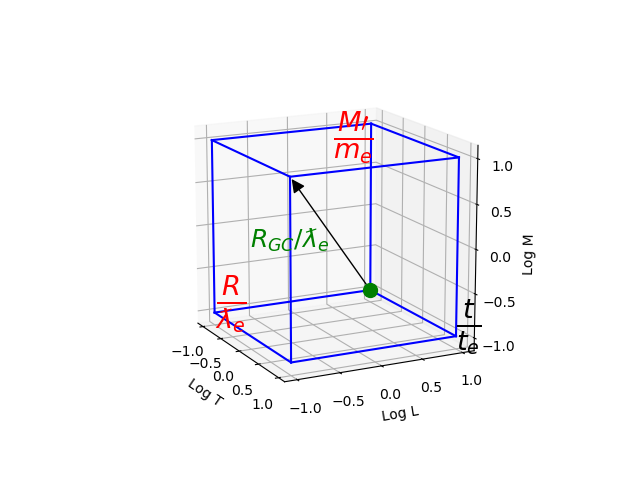
\includegraphics[width=8cm,height=6.5cm]{./figures/triaxis.png}
\caption{Tri-axis superframe structure. Geo dimensional property of the couple Universe-Grandcosmos. In a 3-D super-space , length, time and mass ratios are considered as vectors. The ratio of Grandcosmos radius by the Compton electron wavelength appears as the norm of the vector using for length and time projections the same ratio, that of the Hubble radiusby the electron Compton wavelength2, and for mass ratio that of $M\prime$ by the electron mass; $M\prime$ being the critical mass in the grandcosmos reduced spherical hologram. }
\end{figure}

\section{Citations}
\markright{Bizouard, Flawisky, Gayral, Grosmann, Gueroult, Kotov, Sanchez, Veysseyre. Back to Cosmos}

A single citation is here: \cite{eddy}. Multiple citations are as follows \cite{bondi,Pez,La2}. A citation containing a comment is \cite[see p.\,5]{eddy}

%%%%%%%% the \cite{eddy} command generates citation number proceeded from
%%%%%%%% the label \bibitem{eddy} in the bibliography list

\section*{Acknowledgements}

This research would not have been possible without ...
"Francis M. Sanchez, Valery A. Kotov, Michel Grosmann, Dominique Weigel, Renee
Veysseyre, Christian Bizouard, Nicolas Flawisky, Denis Gayral, Laurent Gueroult."
%
\begin{flushright}\footnotesize
Submitted on Month Day, Year / Accepted on Month Day, Year
\end{flushright}


\begin{thebibliography}{99}\footnotesize

\bibitem{eddy} Eddington A.\,S. The mathematical
theory of relativity. Cambridge University Press,
Cambridge, 1924. % Here is referred book

\bibitem{bondi}  Bondi~H. Negative mass in General 
Relativity. \textit{Review of Modern Physics}, 1957, 
v.\,29\,(3), 423--428. % Here is referred article

\bibitem{Pez} Pezzaglia W. Physical applications of 
generalized Clifford Calculus: Papatetrou equations 
and metamorphic curvature. arXiv: gr-qc/9710027. 
% Here is referred electronic publication

\bibitem{La2}  Lambiase G., Papini G.,  Scarpetta G. 
Maximal acceleration corrections to the Lamb shift
of one electron atoms. \textit{Nuovo Cimento}, 
v.\,B112, 1997, 1003. arXiv: hep-th/9702130.
% Here is double paper-electronic published article

\bibitem{1} Carr B.J. and Rees M. J. , “The anthropic principle and the structure of the physical world”,
Nature 278, 605-612 (1979). % Here is referred book

\bibitem{2} Francis M. Sanchez. Coherent Cosmology Vixra.org,1601.0011. Springer International Publishing AG
2017. A. Tadjer et al. (eds.), Quantum Systems in Physics, Chemistry, and Biology, Progress in
Theoretical Chemistry and Physics 30, pp. 375-407. DOI 10.1007/978-3-319-50255-7-23. % Here is referred book

\bibitem{3} Bonvin V. Holicow, New cosmograil time delays of HE 0435-1223, arXiv: 1607.01790v2
(2016). % Here is referred book

\bibitem{4} Sanchez F.M., V. A. Kotov and C. Bizouard C. Towards a synthesis of two cosmologies: the
steady-state flickering Universe., \textit{Journal of Cosmology}, v.\, 17, 7225-7237 (2011). % Here is referred book

\bibitem{5} Bousso R., “The Holographic Principle”, \textit{Review of Modern Physics}, v.\, 74, p.834 (2002).[7] Duplantier B. Introduction à l'effet Casimir, Séminaire Poincaré 1 (2002), 41-54.. % Here is referred book

\bibitem{6} Damour T. The Entropy of Black Hole: a Primer. Séminaire Poincaré 2 (2003), 100 (89-115. % Here is referred book

\bibitem{7} Carr B.J. and Rees M. J. , “The anthropic principle and the structure of the physical world”,
\textit{Nature} 278, 605-612 (1979). % Here is referred book

\bibitem{8} Kotov V. A. and Lyuty V. M., “The 160-min. Periodicity in the optical and X-ray observations of
extragalactic objects.” Compt. Rend. Acad. Sci. Paris 310, Ser. II, 743-748 (1990). Fossat, E.,
Boumier, P., Corbard, T., et al., 2017. Astron. Astrophys., 604, A40, 1; DOI: 10.1051/0004-
6361/201730460. Grec, G., Fossat, E., 1979. Astron. Astrophys., 77, 351. Kotov, V.A., 2013.
Izv. Krym. Astrofiz. Obs., 109(1), 232. Kotov, V.A., 2018. Earth Moon Planets, 122(1), 43;
DOI:10.1007/s11038-018-9520-6. Sevin E., 1946. Compt. Rend. Acad. Sci. Paris, 222, 220.
Kotov, V.A., 2018. Motion of the fast exoplanets. Astrophys. Space Sci. 363(3), 1-5; DOI:
10.1007/s10509-018-3278-1. % Here is referred book

\bibitem{9} \textit{Review of Particle Physics}. Particle Data Group, Phys. Rev. D98, 030001 (2018)

\bibitem{10} Quinn T, Speake C, Parks H, Davis R. 2014 The BIPM measurements of the Newtonian
constant of gravitation, G. Phil.Trans. R. Soc. A372: 20140032. % Here is referred book

\bibitem{11} Sanchez F.M., “Towards the grand unified Holic Theory”. \textit{Current Issues in Cosmology}. Ed. J.-C.
Pecker and J. Narlikar. Cambridge Univ. Press, 257-260 (2006).

\bibitem{12} Kotov V. A. and Sanchez F.M., Solar 22 years cycle, \textit{Astrophysics and Space Science}, v.\, 362,
Issue 1, article id.6, 6 pp. (2017).

\bibitem{13} Tifft, W. G. (2006). "Redshift periodicities, The Galaxy-Quasar Connection". \textit{Astrophysics and
Space Science} v.\,285 (2):429.

\bibitem{14} Arp H., The origin of Companion Galaxies. \textit{Astrophysical Journal}, 496, 661-669 (1998).

\bibitem{15} Nieto M., and Anderson J., Using Early Data to Illuminate the Pioneer Anomaly, Pi Class.
Quant. Grav. 22 (2005) 5345-5354. arXiv:ge-qc/0507052.

\bibitem{16} Borcherds, Richard, Monstruous Moonshine and Monstruous Lie Superalgebras. Invent.
Math., 109: 405–444, (1992).

\bibitem{17} Nieto M., and Anderson J., Using Early Data to Illuminate the Pioneer Anomaly, Pi Class.
Quant. Grav. 22 (2005) 5345-5354. arXiv:ge-qc/0507052.

\bibitem{18} I. Bars, Gauge Duality, Conformal Symmetry, and Space-Time with Two Times, Phys. Rev. D
58 (1998) hep-th/9803188.

\bibitem{19} Cartan H. Démonstration homologique des théorèmes de périodicité de Bott, I. Séminaire
Henri Cartan, Tome 12 (1959-1960) no. 2, Exposé no. 16, p. 1-16.

\bibitem{20} Preskill, John. Do Black Holes Destroy Information? International Symposium on Black Holes,
Membranes, Wormholes, and Superstrings. arXiv:hep-th/9209058. (1992).

\bibitem{21} Nikolic, Hrvoje. "Resolving the black-hole information paradox by treating time on an equal
footing with space". Physics Letters B. 678 (2): 218–221. arXiv:0905.0538. (2009)

\bibitem{22} Koide Y., Fermion-Boson Two-Body Model of Quarks and Leptons and Cabibbo Mixing Lett.
Nuovo Cimento 34, 201 (1982)

\bibitem{23} J. H. Conway and S. P. Norton, Monstrous Moonshine, Bull. London Math. Soc. 11 (1979), no.
3, 308–339

\bibitem{24} Atiyah M. The fine-structure constant, 4th Heidelberg Laureate Forum conference (2018).
https://www.heidelberg-laureate-forum.org/blog/video/lecture-monday-september-24-2018-sir-michael-francis-atiyah/

\bibitem{25} Polchinski J., String Theory, Vol 1, p. 22 (Cambridge University Press, 1998)

\bibitem{26} R. Chauvin, Le Darwinisme ou la fin d'un mythe, ed. du Rocher, 1997

\bibitem{27} Woit P. Not Even Wrong: The Failure of String Theory and the Search for Unity in Physical
Law. Basic books, 2006

\bibitem{28} Larin S.A, Quantum Chromodynamics with massive gluons. ArXiv:1304.8107, (2013)

\bibitem{29} Durham I.T. 2006, Sir Arthur Eddington and the Foundations of Modern Physics arXiv:quant-
ph/0603146v1 p.111.

\bibitem{30} Widom A. Et al, Electromagnetic signals from Bacteria DNA, arXiv: 1104.311v2, 2012

\bibitem{31} Salingaros N., Some Remarks on the Algebra of Eddington's E Numbers. Foundations of
Physics, June 1985, Volume 15, 6, pp 683–691

\bibitem{32} Weigel D., Veysseyre R and Carel C. Sur les symboles du groupe d'espace d'une wüstite de tri-
incommensurabilité cubique est sur les groupes de Bravais de sa famlille cristalline dans
l'espace euclidien à six dimensions. C.R. Acad. Sci. Paris, t. 305, Série II, p. 349-352 (1987)

\bibitem{33} Atiyah M., private communication (December 2018)

\bibitem{34} {article,
author {Gaudeau de Gerlicz, Claude and Antoine, Mathias and Bobola, Philippe and Flawisky, Nicolas and Hebras, Xavier and Mundedi, Musa},
year {2013},
month {09},
pages {336-340},
title {Emergence of a New Quantum Mechanics by Multivalued Logic},
doi {10.1142/9789814504782-0036}
}

\bibitem{35} {dataset,
author = {Sternheimer, Joël},
year = {1994},
month = {05},
pages = {},
title = {Ondes échelle II. Aperçu de théorie non-linéaire et d'applications biologiques.}
}

\bibitem{36}{article,
author = {Maruani, Jean},
year = {2015},
month = {12},
pages = {n/a-n/a},
title = {The Dirac Electron: From Quantum Chemistry to Holistic Cosmology},
volume = {63},
journal = {Journal of the Chinese Chemical Society},
doi = {10.1002/jccs.201500374}
}

\end{thebibliography}
\vspace*{-6pt}
\centerline{\rule{72pt}{0.4pt}}
}


\end{document}
